\subsection{Iterative Methods for Linear Systems}

\frame{
\begin{itemize}
\item Linear systems with as many as $100,000$ variables often arise in the solution of partial differential equations. 
\vspace{3mm}
\item The coefficient matrices for these systems are sparse; that is, a large percentage of the entries of the coefficient matrix are zero. 
\vspace{3mm}
\item If there is a pattern to the nonzero entries (i.e., tridiagonal systems), then an iterative process provides an efficient method for solving these large systems. 
\end{itemize}
}

\frame{
\begin{block}{}
\begin{itemize}
\item The goal of this section is to extend some of the iterative methods introduced in Chapter 1 to higher dimensions. 
\vspace{5mm}
\item We consider an extension of fixed-point iteration that applies to systems of linear equations. 
\end{itemize}
\end{block}
\begin{center}
$\Downarrow$
\end{center}
\begin{block}{}
\begin{itemize}
\item {\Large Jacobi Iteration}
\item {\Large Gauss-Seidel Iteration}
\end{itemize}
\end{block}
}

\frame{
%\frametitle{Jacobi Iteration}
\frametitle{Example 2.9.}
Consider the system of equations
\begin{equation*}
\begin{array}{r c r c r c r}
4x & - &   y & + & z & = & 7 \\
4x & - & 8y & + & z & = & -21 \\
-2x & + & y & + & 5z & = & 15
\end{array}
\end{equation*}
\begin{center}
$\Downarrow$
\end{center}
These equations can be written in the form
\begin{equation*}
\begin{array}{l c l}
x & = & \frac{7+y-z}{4} \\
y & = & \frac{21+4x+z}{8} \\
z & = & \frac{15+2x-y}{5}
\end{array}
\end{equation*}
}

\frame{
\begin{center}
$\Downarrow$
\end{center}
This suggests the following Jacobi iterative process:
\begin{equation*}
\begin{array}{l c l}
x_{k+1} & = & \frac{7+y_{k}-z_{k}}{4} \\
y_{k+1} & = & \frac{21+4x_{k}+z_{k}}{8} \\
z_{k+1} & = & \frac{15+2x_{k}-y_{k}}{5}
\end{array}
\end{equation*}
\begin{center}
$\Downarrow$
\end{center}
Let us show that if we start with $P_0 = (x_0, y_0, z_0) = (1, 2, 2)$, then the iteration in this equation appears to converge to the solution (2, 4, 3).
\begin{figure}
\begin{center}
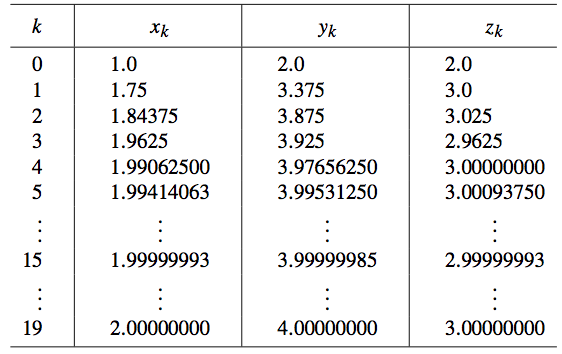
\includegraphics[width=55mm]{chap-2/tab_3-2.png}
\end{center}
\end{figure}
}


\frame{
\begin{block}{}
\begin{itemize}
\item Sometimes the Jacobi method does not work. 
\item Let us experiment and see that a rearrangement of the original linear system can result in a system of iteration equations that will produce a divergent sequence of points. 
\end{itemize}
\end{block}
}

\frame{
\frametitle{Example 2.10.}
Let the linear system in example 2.9 be rearranged as follows:
\begin{equation*}
\begin{array}{r c r c r c r}
-2x & + & y & + & 5z & = & 15 \\
4x & - &   y & + & z & = & 7 \\
4x & - & 8y & + & z & = & -21
\end{array}
\end{equation*}
These equations can be written in the form
\begin{equation*}
\begin{array}{l}
x = \frac{-15 + y + 5z}{2} \\
y = \frac{21 +4x + z}{8}  \\
z = 7 - 4x +y. 
\end{array}
\end{equation*}
This suggests the following Jacobi iterative process:
\begin{equation*}
\begin{array}{l}
x_{k+1} = \frac{-15 + y_k + 5z_k}{2} \\
y_{k+1} = \frac{21 +4x_k + z_k}{8}  \\
z_{k+1} = 7 - 4x_k +y_k. 
\end{array}
\end{equation*}
}

\frame{
\begin{itemize}
\item See that if we start with $P_0 = (x_0, y_0, z_0) = (1,2,2)$, then the iteration using (2.38) will diverge away from the solution (2,4,3). 
\item Substitute $x_0 = 1$, $y_0 = 2$, and $z_0 = 2$ into the right-hand side of each equation in (2.38) to obtain the new values $x_1$,$y_1$, and $z_1$ : 
\begin{equation*}
\begin{array}{l}
x_1 = \frac{-15 + 2 + 10}{2} = -1.5 \\ 
y_1 = \frac{21 + 4 + 2}{8} = 3.375 \\
z_1 = 7 - 4 + 2 = 5.00. 
\end{array}
\end{equation*}
\end{itemize}
}

\frame{
\begin{itemize}
\item The new point $P_1 = (-1.5,3.375,5.00)$ is farther away from the solution (2,4,3) than $P_0$. 
\item Iteration using the equations in (2.38) produces a divergent sequence (see Table 2.2). 
\end{itemize}
\begin{figure}
\begin{center}
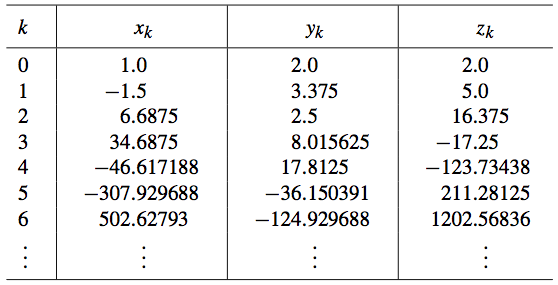
\includegraphics[width=80mm]{chap-2/tab_3-3.png}
\end{center}
\end{figure}
}


\frame{
\frametitle{Gauss-Seidel Iteration}
\begin{itemize}
\item Sometimes the convergence can be speeded up. 
\item Observe that the Jacobi iterative process (2.35) yields three sequences $\{ x_k\} $, $\{ y_k\} $, and $\{ z_k\} $ that converge to $2$, $4$ and $3$, respectively (see Table 2.1).
\item Since $x_{k+1}$ is expected to be a better approximation to $x$ than $x_k$, it seems reasonable that $x_{k+1}$ could be used in place of $x_k$ in the computation of $y_{k+1}$ \item Similarly, $x_{k+1}$ and $y_{k+1}$ might be used in the computation of $z_{k+1}$. 
\item The next example shows what happens when this is applied to the equations in Example 2.9. 
\end{itemize}
}

\frame{
\frametitle{Example 2.11.}
Consider the system of equations given in example 2.9 and the Gauss-Seidel iterative process suggested by :
\begin{equation*}
\begin{array}{l c l}
x_{k+1} & = & \frac{7+y_{k}-z_{k}}{4} \\
y_{k+1} & = & \frac{21+4x_{k+1}+z_{k}}{8} \\
z_{k+1} & = & \frac{15+2x_{k+1}-y_{k+1}}{5}
\end{array}
\end{equation*}
\begin{center}
$\Downarrow$
\end{center}
See that if we start with $P_0 = (x_0, y_0, z_0) = (1, 2, 2)$, then iteration  will converge to the solution $(2, 4, 3)$.
}

\frame{
Substitute $y_0 = 2$ and $z_0 = 2$ into the first equation  and obtain
\begin{equation*}
x_1 = \frac{7+2-2}{4} = 1.75
\end{equation*}
Then substitute $x_1 = 1.75$ and $z_0 = 2$ into the second equation and get
\begin{equation*}
y_1 = \frac{21 + 4(1.75) + 2}{8} = 3.75
\end{equation*}
Finally, substitute $x_1 = 1.75$ and $y_1 = 3.75$ into the third equation to get
\begin{equation*}
z_1 = \frac{15 + 2(1.75) - 3.75}{5} = 2.95
\end{equation*}
This iteration generates a sequence $\left\{ P_k \right\}$ that converges to $(2, 4, 3)$.
\begin{figure}
\begin{center}
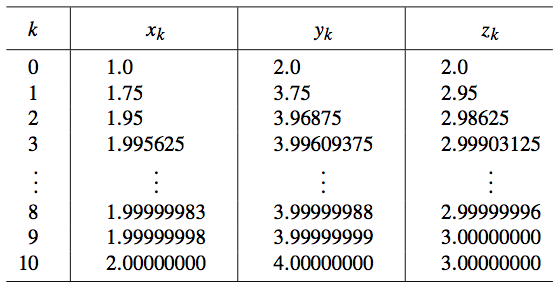
\includegraphics[width=60mm]{chap-2/tab_3-4.png}
\end{center}
\end{figure}
}

\frame{
\begin{block}{Definition 2.4.}
A matrix $A$ of dimension $N \times N$ is said to be strictly diagonally dominant provided that
\begin{equation*}
\left| a_{k, k}\right| > \sum^{N}_{j=1, j\ne k} \ \ \ for \ \ k = 1, 2, \ldots, N 
\end{equation*}
\end{block}
This means that in each row of the matrix the magnitude of the element on the main diagonal must exceed the sum of the magnitudes of all other elements in the row. \\
The coefficient matrix of the linear system (3.33) in Example 2.9 is strictly diagonally dominant because 
\begin{equation*}
\begin{array}{l l}
In \ row \ 1 : & |4|   > |-1| + |1| \\
In \ row \ 2 : & |-8| > |4|   + |1| \\
In \ row \ 3 : & |5|   > |-2| + |1| 
\end{array}
\end{equation*}
}

\frame{
All the rows satisfy relation (2.40) in Definition 2.4; therefore, the coefficient matrix A for the linear system (3.33) is strictly diagonally dominant.  \\
The coefficient matrix $A$ of the linear system (3.36) in Example 2.10 is not strictly diagonally dominant because 
\begin{equation*}
\begin{array}{l l}
In \ row \ 1 : & |-2| < |1| + |5| \\
In \ row \ 2 : & |-8| > |4| + |1| \\
In \ row \ 3 : & |1|   < |4| + |-1| 
\end{array}
\end{equation*}
\begin{block}{}
Rows $1$ and $3$ do not satisfy relation (2.40) in Definition 2.4; therefore, the coefficient matrix $A$ for the linear system (2.36) is not strictly diagonally dominant. 
\end{block}
}

\frame{
We now generalize the Jacobi and Gauss-Seidel iteration processes. 
Suppose that the given linear system is
\begin{equation*}
\begin{array}{c c c c c c c c c c c c c}
a_{1,1} x_1 & + & a_{1,2} x_2 &  + & \cdots & + & a_{1,j} x_j &  + & \cdots & + & a_{1,N} x_N & = & b_1 \\
a_{2,1} x_1 & + & a_{2,2} x_2 &  + & \cdots & + & a_{2,j} x_j & + & \cdots & + & a_{2,N} x_N & = & b_2 \\
\vdots       &     & \vdots        &     &             &    &    \vdots   &    &             &    &  \vdots        &    & \vdots \\
a_{j,1} x_1 & +  & a_{j,2} x_2  & +  & \cdots & + & a_{j,j} x_j  & + & \cdots & + & a_{j,N} x_N  & = & b_3 \\
\vdots       &     & \vdots        &     &             &    &    \vdots   &    &              &    &  \vdots        &    & \vdots \\
a_{N,1} x_1 & + & a_{N,2} x_2 & + & \cdots & + & a_{N,j} x_j & + & \cdots & + & a_{N,N} x_N & = & b_N
\end{array}
\end{equation*}
\begin{itemize}
\item Let the $k$th point be $P_k = \left( x_1^{(k)}, x_2^{(k)}, \ldots, x_j^{(k)}, \ldots, x_N^{(k)}  \right)$; 
\item then the next point is $P_{k+1} = \left( x_1^{(k+1)}, x_2^{(k+1)}, \ldots, x_j^{(k+1)}, \ldots, x_N^{(k+1)}  \right)$. 
\item The superscript $(k)$ on the coordInates of $P_k$ enables us to identify the coordinates that belong to this point. 
\item The iteration formulas use row $j$ of (2.41) to solve for $x_j^{k+l}$ in terms of a linear combination of the previous values $x_1^{(k)}$, $x_2^{(k)}$, $\ldots$, $x_j^{(k)}$, $\ldots$, $x_N^{(k)}$:
\end{itemize}
}

\frame{
\begin{block}{}
Jacobi iteration uses all old coordinates to generate all new coordinates, whereas Gauss-Seidel iteration uses the new coordinates as they become available:
\end{block}
\begin{itemize}
\item Jacobi iteration:
\begin{equation*}
x_j^{(k+1)} = \frac{b_j - a_{j,1} x^{(k)}_1 - \cdots - a_{j, j-1} x^{(k)}_{j-1} - a_{j, j+1} x^{(k)}_{j+1} - \cdots - a_{j,N} x^{(k)}_N}{a_{j,j}}
\end{equation*}
for $j = 1, 2,  \ldots , N$.
\item Gauss-Seidel iteration:
\begin{equation*}
x_j^{(k+1)} = \frac{b_j - a_{j,1} x^{(k+1)}_1 - \cdots - a_{j, j-1} x^{(k+1)}_{j-1} - a_{j, j+1} x^{(k)}_{j+1} - \cdots - a_{j,N} x^{(k)}_N}{a_{j,j}}
\end{equation*}
for $j = 1, 2,  \ldots , N$.
\end{itemize}
}

\frame{
\begin{block}{Theorem 2.7 (Jacobi Iteration).} 
Suppose that $A$ is a strictly diagonally dominant matrix. 
Then $AX = B$ has a unique solution $X = P$. 
Iteration  will produce a sequence of vectors $\{ P_k \}$ that will converge to $P$ for any choice of the starting vector $P_0$.
\end{block}
\begin{itemize}
\item It can be proved that the Gauss-Seidel method will also converge when the matrix $A$ is strictly diagonally dominant. 
\item In many cases the Gauss-Seidel method will converge faster than the Jacobi method; hence it is usually preferred (compare Examples 2.9 and 2.11). 
\item It is important to understand the slight modification of formula (2.42) that has been made to obtain formula (2.43). 
\item In some cases the Jacobi method will converge even though the Gauss-Seidel method will not. 
\end{itemize}
}

\frame{
\frametitle{Convergence}
A measure of the closeness between vectors is needed so that we can determine if $\{ P_k \}$ is converging to $P$. 
The Euclidean distance\footnote{see Section 2.1} between $P = (x_1, x_2, \ldots, x_N )$ and $Q = (y_1, y_2, \ldots, y_N )$ is
\begin{equation*}
\left| \left| P -Q \right| \right| = \left( \sum_{j=1}^N \left( x_j - y_j \right)^2 \right)^{1 \slash 2}
\end{equation*}
Its disadvantage is that it requires considerable computing effort. 
Hence we introduce a different norm,
\begin{equation*}
\left| X \right|_1 = \sum_{j=1}^N \left| x_j  \right| 
\end{equation*}
}

\frame{
\begin{itemize}
\item The following result ensures that $|| X ||_1$ has the mathematical structure of a metric and hence is suitable to use as a generalized "distance formula." 
\vspace{5mm}
\item From the study of linear algebra we know that on a finite-dimensional vector space all norms are equivalent; that is, if two vectors are close in the $||\ast||_1$ norm, then they are also close in the Euclidean norm $||\ast||$. 
\end{itemize}
}

\frame{
\begin{block}{Theorem 2.8.} 
Let $X$ and $Y$ be $N$-dimensional vectors and $c$ be a scalar. 
Then the function $|| X ||_1$ has the following properties:
\begin{equation*}
\begin{array}{r}
|| X ||_1 \ge 0 \\
|| X ||_1 = 0 \ \ if \ \ and  \ \ only \ \ if \ \ X = 0 \\  
|| cX ||_1 = |c| || X ||_1 \\
|| X + Y ||_1 \le || X ||_1 + || Y ||_1
\end{array}
\end{equation*}
\end{block}
Proof. \\
For each $j$, the triangle inequality for real numbers states that $|x_j + y_j| \le |x_j| + |y_j|$. 
Summing these yields inequality:
\begin{equation*}
|| X + Y ||_1 = \sum_{j=1}^N |x_j + y_j| \le \sum_{j=1}^N |x_j| + \sum_{j=1}^N |y_j| =  || X ||_1 + || Y ||_1
\end{equation*}
}

\frame{
\begin{block}{Definition 2.5.}
Suppose that $X$ and $Y$ are two points in $N$-dimensional space. 
We define the distance between $X$ and $Y$ in the  $||\ast||_1$ norm as
\begin{equation*}
|| X - Y ||_1 = \sum_{j=1}^N |x_j - y_j|
\end{equation*}
\end{block}
Example 2.12. \\
Determine the Euclidean distance and $||\ast||_1$ distance between the points $P = (2, 4, 3)$ and $Q = (1.75, 3.75, 2.95)$.
The Euclidean distance is
\begin{equation*}
\left| \left| P -Q \right| \right| = \left( (2 - 1.75)^2 + (4 - 3.75)^2 + (3 - 2.95)^2 \right)^{1/2} = 0.3570
\end{equation*}
the  $||\ast||_1$  distance is
\begin{equation*}
\left| \left| P -Q \right| \right|_1 = |2 - 1.75| + |4 - 3.75| + |3 - 2.95| = 0.55
\end{equation*}
}

